\documentclass[aspectratio=169,xcolor=table]{beamer}
\usepackage[utf8]{inputenc}
\usepackage[T1,T5]{fontenc}
\usepackage{amsmath,amssymb,booktabs,array,graphicx}

\definecolor{Primary}{HTML}{111B88}
\definecolor{Secondary}{HTML}{101659}
\definecolor{Accent}{HTML}{F2A900}
\definecolor{SoftBlue}{HTML}{EAF2F8}
\definecolor{TextGray}{HTML}{4D5966}
\definecolor{RiskRed}{HTML}{A23B3B}
\definecolor{GoodGreen}{HTML}{26734D}
\mode<presentation>{\usetheme{Madrid}\usecolortheme{default}\setbeamertemplate{navigation symbols}{}}
\setbeamercolor{structure}{fg=Primary}
\setbeamercolor{frametitle}{fg=white,bg=Primary}
\setbeamercolor{title}{fg=white,bg=Primary}
\setbeamercolor{block body}{fg=black,bg=SoftBlue}
\setbeamercolor{block body alerted}{fg=black,bg=Accent!12}
\setbeamercolor{section in head/foot}{fg=white,bg=Primary}
\setbeamercolor{author in head/foot}{fg=white,bg=Secondary}
\setbeamercolor{date in head/foot}{fg=white,bg=Primary}
\setbeamerfont{section in head/foot}{size=\tiny,series=\bfseries}
\setbeamerfont{author in head/foot}{size=\scriptsize}
\setbeamerfont{date in head/foot}{size=\scriptsize,series=\bfseries}
\setbeamerfont{frametitle}{series=\bfseries}
\setbeamerfont{title}{series=\bfseries}
\newcommand{\decklabel}{Contextual ASR -- 23/10/2026}
\setbeamertemplate{itemize item}{\color{Secondary}$\blacktriangleright$}
\setbeamertemplate{itemize subitem}{\color{Accent}$\bullet$}
\setbeamertemplate{headline}{\leavevmode\begin{beamercolorbox}[wd=\paperwidth,ht=2.7ex,dp=1.1ex,leftskip=.35cm,rightskip=.35cm]{section in head/foot}\insertsectionnavigationhorizontal{\dimexpr\paperwidth-.70cm\relax}{}{}\end{beamercolorbox}}
\setbeamertemplate{footline}{\leavevmode\hbox{\begin{beamercolorbox}[wd=.55\paperwidth,ht=2.6ex,dp=1ex,leftskip=.35cm,rightskip=.20cm]{section in head/foot}\usebeamerfont{section in head/foot}\insertsectionhead\end{beamercolorbox}\begin{beamercolorbox}[wd=.27\paperwidth,ht=2.6ex,dp=1ex,center]{author in head/foot}\usebeamerfont{author in head/foot}\decklabel\end{beamercolorbox}\begin{beamercolorbox}[wd=.18\paperwidth,ht=2.6ex,dp=1ex,rightskip=.35cm plus1fil]{date in head/foot}\usebeamerfont{date in head/foot}\hfill\insertframenumber\,/\,\inserttotalframenumber\end{beamercolorbox}}}
\newcommand{\hi}[1]{\textcolor{Primary}{\textbf{#1}}}
\newcommand{\bad}[1]{\textcolor{RiskRed}{\textbf{#1}}}
\newcommand{\good}[1]{\textcolor{GoodGreen}{\textbf{#1}}}
\newcommand{\src}[1]{{\tiny\color{TextGray}[#1]}}
\newcommand{\ra}{$\rightarrow$}

\title{Bias list lớn cho SpeechLLM: chọn từ đã gần trần, nút thắt đang dịch sang chỗ khác}
\subtitle{Vấn đề $\rightarrow$ thí nghiệm $\rightarrow$ insight $\rightarrow$ đề xuất}
\author{Nhóm Contextual ASR}
\institute{}
\date{23/10/2026}
\setbeamertemplate{title page}{\begin{centering}\vspace*{0.10cm}
\includegraphics[height=1.08cm]{imgs/logo.png}\par\vspace{0.32cm}\begin{beamercolorbox}[sep=0.50em,center,rounded=true]{title}\usebeamerfont{title}\inserttitle\par\vspace{0.14cm}{\small\insertsubtitle\par}\end{beamercolorbox}\vspace{0.42cm}{\usebeamerfont{author}\insertauthor\par}\vspace{0.10cm}{\usebeamerfont{institute}\insertinstitute\par}\vfill{\usebeamerfont{date}\insertdate\par}\end{centering}}

\begin{document}
\begin{frame}[plain]\titlepage\end{frame}

% ------------------------------------------------------------------
\section{Tóm tắt}
\begin{frame}{Tóm tắt cả buổi trong 1 slide}
\begin{beamercolorbox}[sep=0.55em,rounded=true]{block body}
\textbf{Câu hỏi:} SpeechLLM được đưa bias list \textbf{lớn, nhiều nhiễu} thì vì sao không dùng được, và làm sao để dùng được?
\end{beamercolorbox}
\vspace{0.1cm}
\small
\begin{itemize}\itemsep2pt
\item \textbf{Vấn đề có thật:} Qwen3-ASR với list 2000 từ có B-WER = \bad{7.40}, y như không có list; chỉ đưa từ đúng: \good{4.01}.
\item \textbf{4 thí nghiệm} \ra{} chọn từ bằng audio lấp được \good{$\sim$75\%} khoảng trống; scorer âm vị \textbf{tốt hơn Hou25}, gần PTC; phần còn thua chủ yếu do \textbf{dữ liệu + tiền xử lý}.
\item \textbf{Insight:} có \hi{2 nút thắt nối tiếp}: \textcircled{\scriptsize 1} chọn đúng từ (đã gần trần) và \textcircled{\scriptsize 2} SpeechLLM dùng đúng từ đã chọn ($\approx$ nửa lỗi còn lại).
\item \textbf{Đề xuất:} scorer trả thêm \hi{vị trí} của từ \ra{} chỉ bias đúng đoạn audio; kiểm trước bằng thí nghiệm \textbf{đo trần} ($\sim$1 ngày GPU).
\end{itemize}
\begin{beamercolorbox}[sep=0.4em,rounded=true]{block body alerted}
\footnotesize\textbf{Cần thầy quyết:} chuyển trọng tâm sang nút thắt \textcircled{\scriptsize 2}? \;·\; SpeechLLM đóng băng hay fine-tune / RL? \;·\; gác hướng ``tự dựng list''? \;·\; tập thứ hai?
\end{beamercolorbox}
\end{frame}

% ------------------------------------------------------------------
\section{Vấn đề}
\begin{frame}{Vấn đề: list càng dài, SpeechLLM càng không dùng được}
\centering
{\small Qwen3-ASR-1.7B, LibriSpeech + list IS21, B-WER test-clean / test-other (thấp = tốt)}\par\vspace{0.2cm}
\footnotesize\setlength{\tabcolsep}{4pt}
\begin{tabular}{lcccccc}
\toprule
List & không list & \textbf{oracle} & N100 & N500 & N1000 & N2000\\
\midrule
B-WER & 7.40 / 16.08 & \good{4.01 / 7.73} & 5.30 / 11.61 & 6.73 / 14.88 & 7.30 / 15.92 & \bad{7.40 / 16.45}\\
\bottomrule
\end{tabular}
\vspace{0.25cm}
\raggedright\normalsize
\begin{itemize}\itemsep4pt
\item List của mỗi câu = từ hiếm đúng ($\sim$2) + N từ nhiễu. Ở \textbf{N2000}, đưa list cũng như không.
\item Hai cách hỏng: từ đúng \textbf{bị loãng} giữa hàng nghìn từ; mô hình \textbf{tự chèn} từ trong list.
\item Đây là điểm chung của Hou25, PTC-Bias, BR-ASR, Huber \& Waibel \src{ta diễn giải}.
\end{itemize}
\vspace{0.1cm}
\begin{beamercolorbox}[sep=0.45em,rounded=true]{block body}
\small\textbf{Giả thuyết ban đầu} (cũng là giả định của các paper trên): nút thắt là \textbf{chọn từ}. Lọc list bằng audio còn vài từ đúng thì SpeechLLM dùng được như oracle.
\end{beamercolorbox}
\end{frame}

\begin{frame}{Hệ thống và hai nút thắt}
\centering
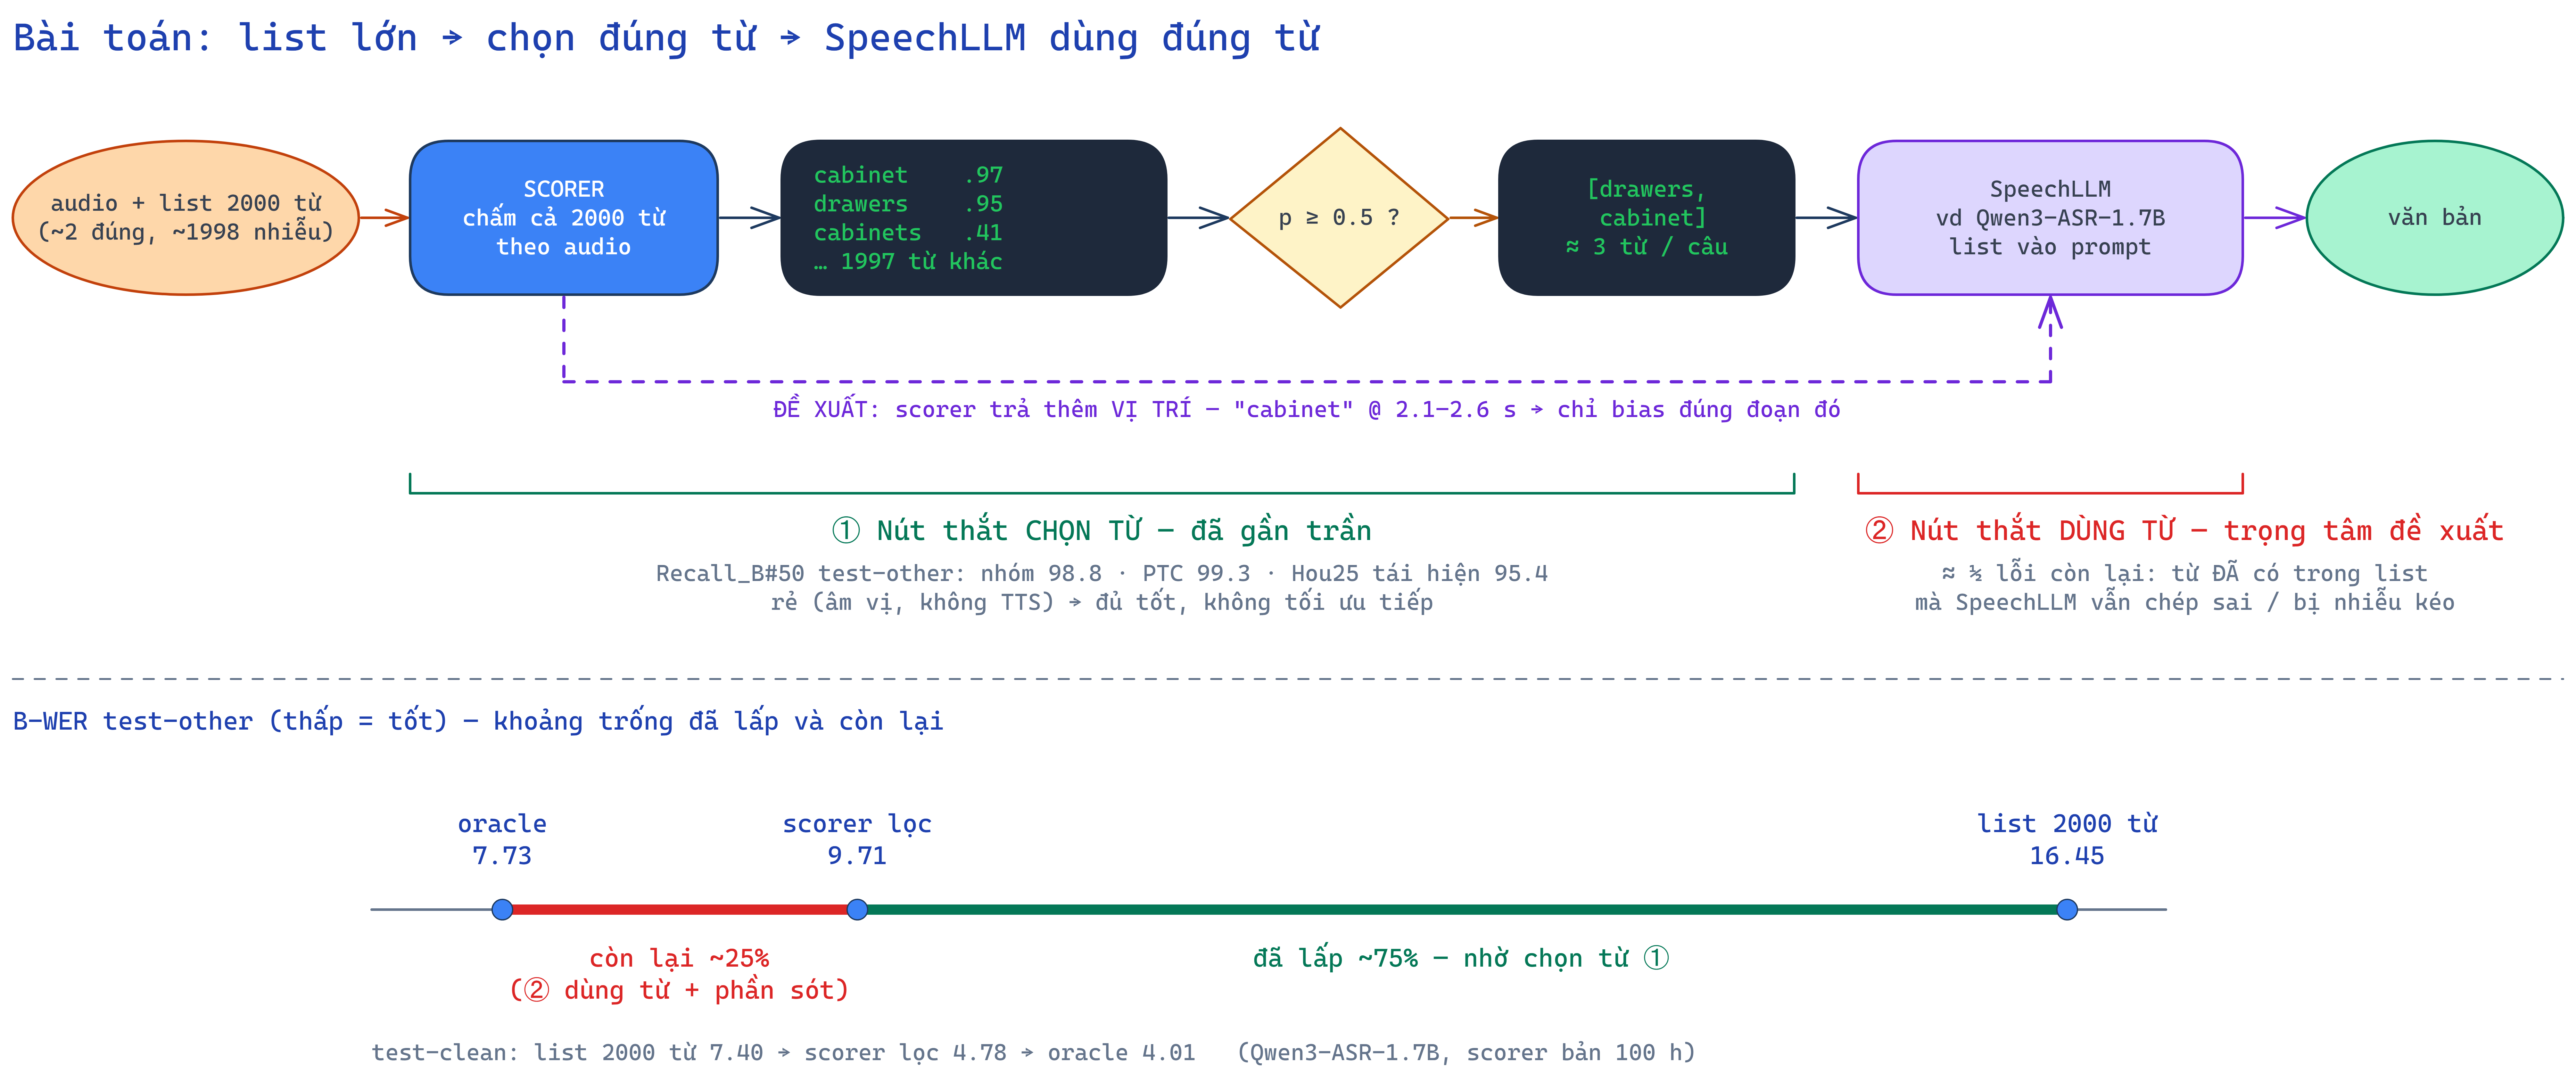
\includegraphics[width=\linewidth,height=0.86\textheight,keepaspectratio]{imgs/pipeline_2bottleneck.png}
\end{frame}

% ------------------------------------------------------------------
\section{Kiến trúc}
\begin{frame}{Scorer: kiến trúc chi tiết (3 biến thể, chỉ khác bước so)}
\centering
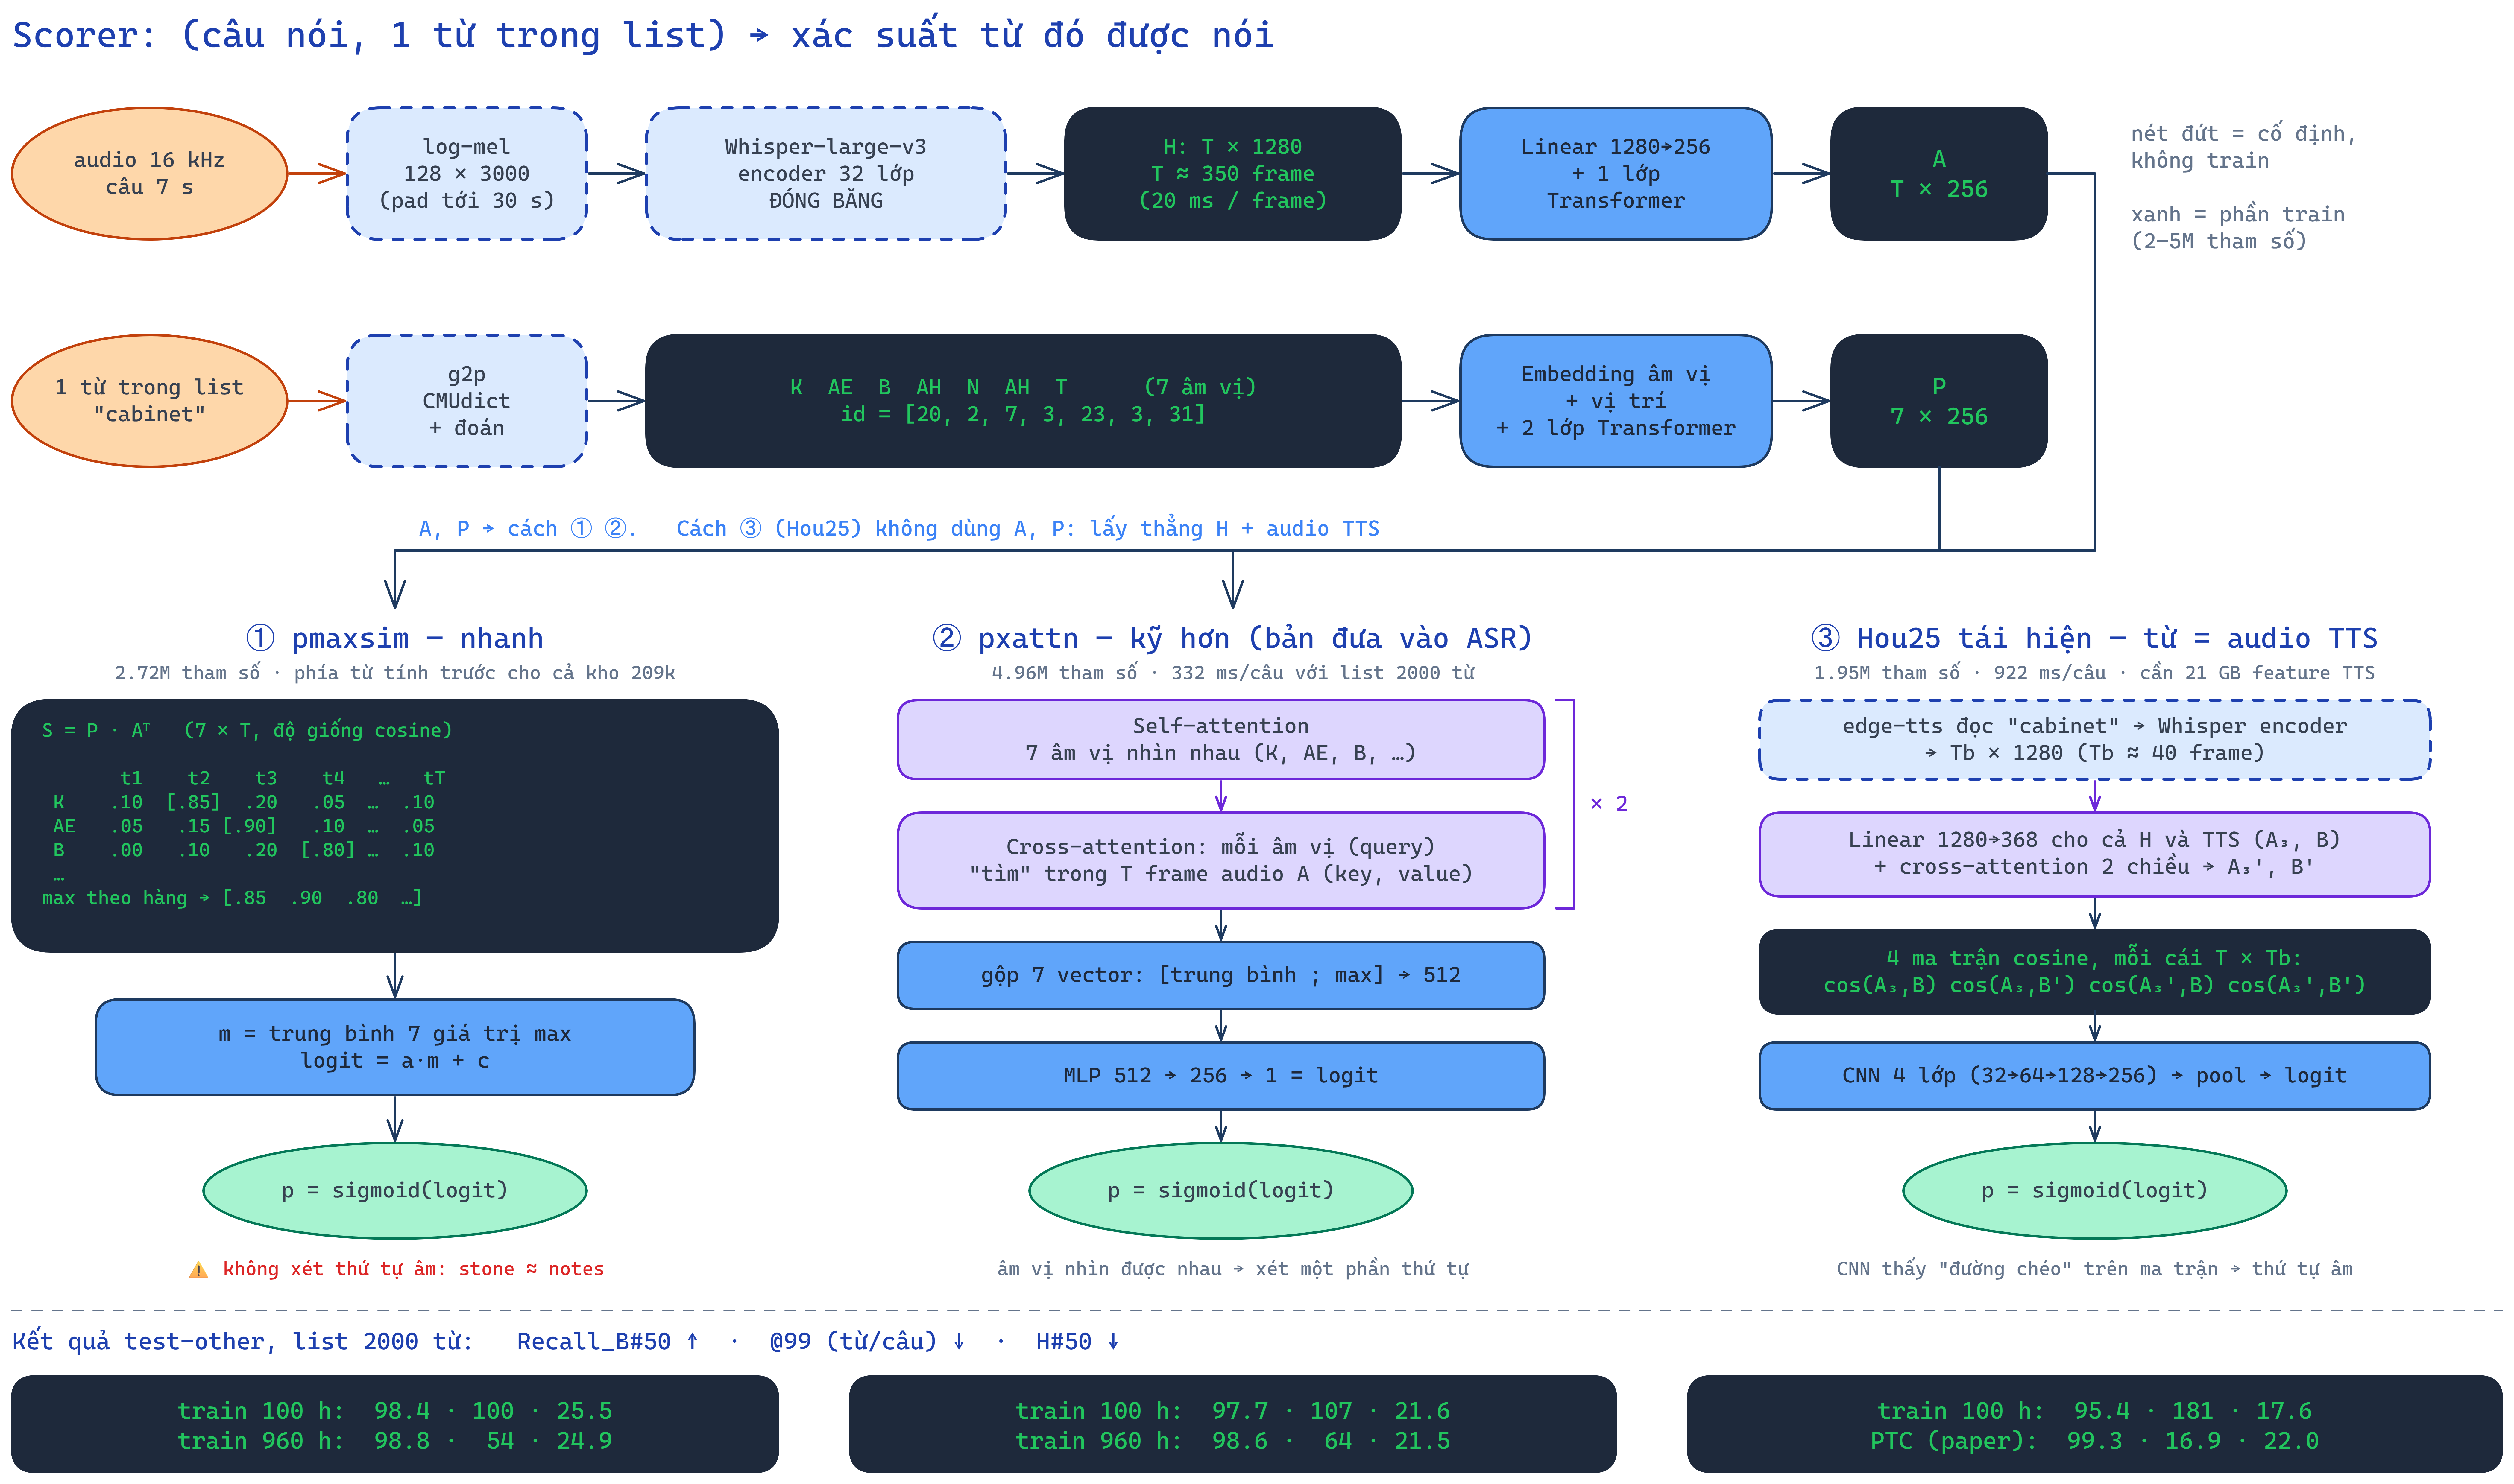
\includegraphics[width=\linewidth,height=0.88\textheight,keepaspectratio]{imgs/scorer_detail.png}
\end{frame}

\begin{frame}{Train scorer}
\begin{columns}[T]
\begin{column}{0.60\textwidth}
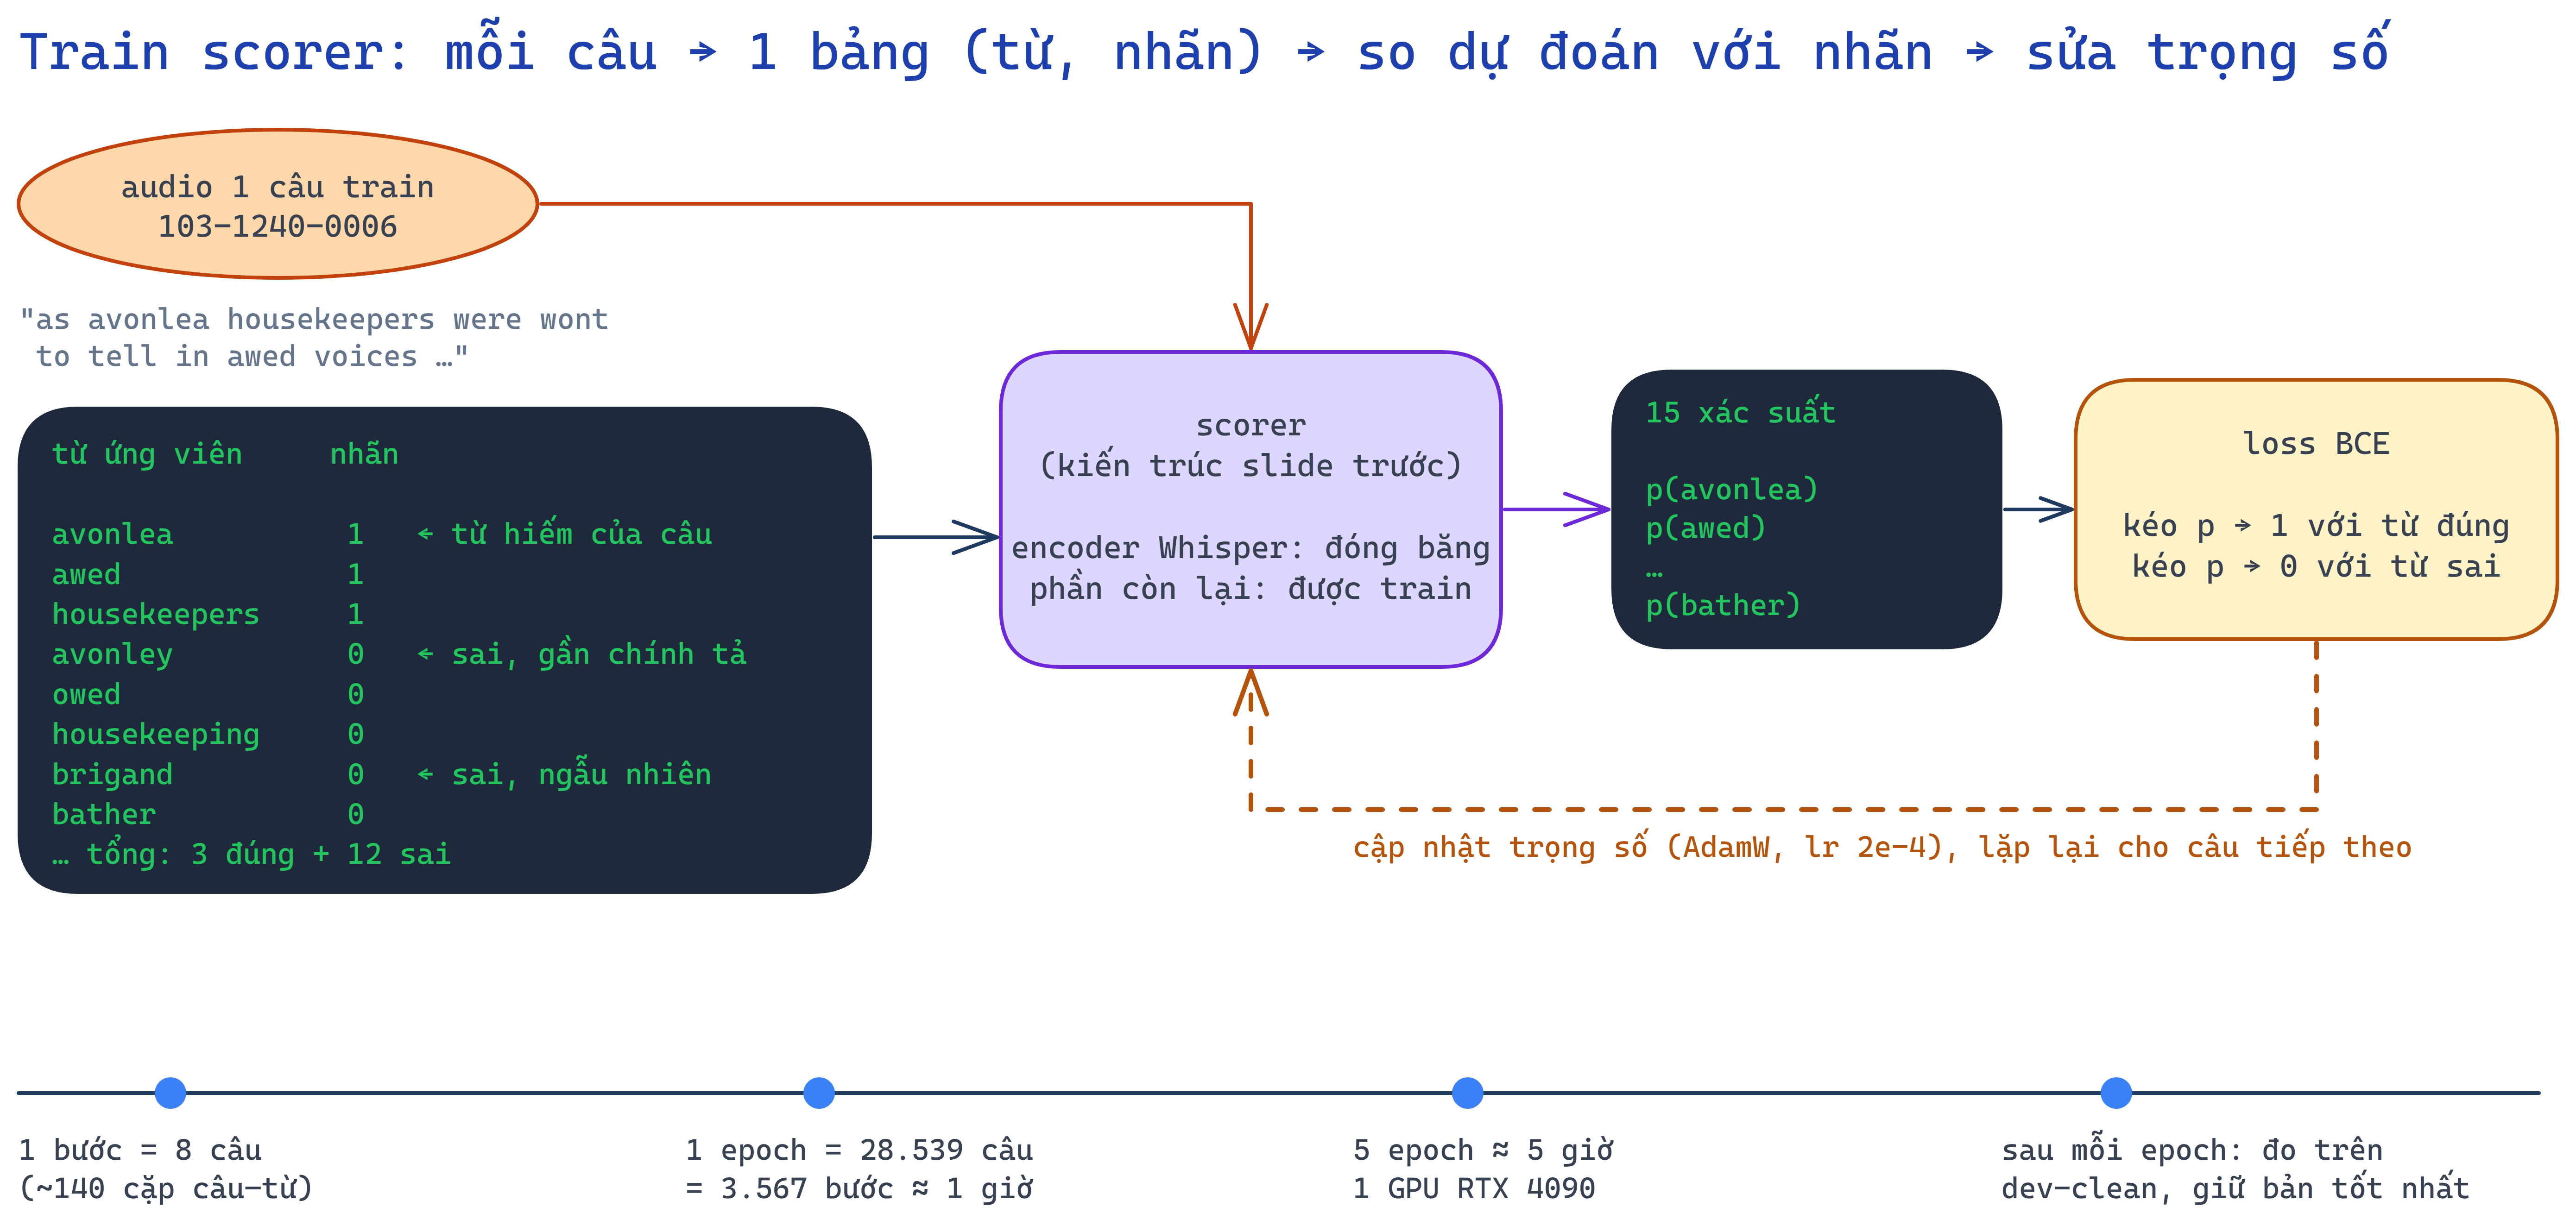
\includegraphics[width=\linewidth]{../2026-10-17/imgs/training.png}
\end{column}
\begin{column}{0.38\textwidth}
\small
\begin{itemize}\itemsep4pt
\item Loss BCE từng cặp (câu, từ); từ sai = 40\% gần chính tả + 60\% ngẫu nhiên trong kho 209k \src{theo Hou25}.
\item Encoder Whisper \textbf{đóng băng}, chỉ train 2--5M tham số.
\end{itemize}
\vspace{0.2cm}
\begin{tabular}{lcc}
\toprule
 & \textbf{100 h} & \textbf{960 h}\\
\midrule
Dữ liệu & clean-100 & + clean-360\\
 & & + other-500\\
Số câu & 28.5k & 281k\\
Giọng khó & không & có\\
Số bước & 17.8k & 35.2k\\
\bottomrule
\end{tabular}\par
\vspace{0.1cm}{\scriptsize Chọn checkpoint trên dev-other, list 2000 từ thật.}
\end{column}
\end{columns}
\end{frame}

% ------------------------------------------------------------------
\section{Thí nghiệm}
\begin{frame}{TN1 -- Lọc list bằng audio có cứu được không?}
\begin{columns}[T]
\begin{column}{0.52\textwidth}
\textbf{Thiết kế:} scorer chấm 2000 từ, giữ từ có $p\geq0.5$ ($\sim$3 từ/câu), so với giữ top-50 như Hou25. Đưa list vào Qwen3-ASR.\par\vspace{0.3cm}
\begin{tabular}{lc}
\toprule
List đưa vào Qwen & B-WER clean / other\\
\midrule
N2000 & 7.40 / 16.45\\
top-50 kiểu Hou25 & 5.71 / 11.57\\
\textbf{lọc theo ngưỡng} & \good{4.78 / 9.71}\\
oracle & 4.01 / 7.73\\
\bottomrule
\end{tabular}
\end{column}
\begin{column}{0.44\textwidth}
\begin{beamercolorbox}[sep=0.55em,rounded=true]{block body alerted}
\textbf{Insight}
\begin{itemize}
\item Lọc bằng audio lấp \good{$\sim$77\%} khoảng trống tới oracle (cả clean và other).
\item \textbf{Ít mà đúng $>$ nhiều mà đủ}: 3 từ tốt hơn hẳn 50 từ.
\end{itemize}
\end{beamercolorbox}
\vspace{0.2cm}
{\scriptsize Scorer bản 100 h (pxattn). Bản 960 h chưa đưa vào ASR.}
\end{column}
\end{columns}
\end{frame}

\begin{frame}{TN2 -- Biểu diễn từ: audio TTS (Hou25) hay âm vị?}
\textbf{Thiết kế:} cùng dữ liệu train 100 h, đo riêng khâu chọn từ bằng metric của PTC / BR-ASR. Test-other, list 2000.\par\vspace{0.25cm}
\centering
\begin{tabular}{lcccc}
\toprule
 & Recall\_B\#50 $\uparrow$ & Recall\_B@99 $\downarrow$ & Recall\_H\#50 $\downarrow$ & tốc độ\\
\midrule
Hou25 tái hiện (TTS + CNN) & 95.4 & 181 & \good{17.6} & 922 ms/câu\\
âm vị -- pmaxsim (nhóm) & \good{98.4} & 100 & 25.5 & 4 ms + encoder\\
âm vị -- pxattn (nhóm) & 97.7 & 107 & 21.6 & 332 ms/câu\\
PTC \src{2609.28727 Bảng 3} & 99.3 & 16.9 & 22.0 & \\
\bottomrule
\end{tabular}\par
\vspace{0.1cm}{\scriptsize \#50: \% từ đúng trong top-50. @99: số từ/câu phải giữ để không sót quá 1\% từ đúng. H\#50: \% từ nghe giống từ đúng lọt top-50.}
\raggedright
\vspace{0.2cm}
\begin{beamercolorbox}[sep=0.5em,rounded=true]{block body alerted}
\textbf{Insight:} âm vị \textbf{tìm từ đúng tốt hơn} Hou25, rẻ hơn $\sim$200 lần, chấm ngay được từ mới (không cần TTS, 21 GB feature).
Hou25 \textbf{ít bị lừa bởi từ nghe giống} hơn \ra{} giả thuyết: CNN nhìn được thứ tự âm \src{chưa kiểm}.
\end{beamercolorbox}
\end{frame}

\begin{frame}{TN3 -- Vì sao còn thua PTC? Loại trừ từng giả thuyết}
\centering\footnotesize
\begin{tabular}{p{3.8cm}p{4.3cm}p{4.9cm}}
\toprule
Giả thuyết & Kiểm bằng & Kết quả\\
\midrule
Điểm lệch giữa các câu & chuẩn hoá điểm theo câu & tệ hơn \ra{} \bad{loại}\\
Loss chưa hợp bài 1/2000 & loss theo list + 200 từ nhiễu & tệ hơn mọi metric \ra{} \bad{loại}\\
Scorer \textbf{nghe kém} giọng khó & xem từ đúng bị rớt & 77--85\% có điểm $<$ 0.3 \ra{} \good{đúng}\\
\textbf{Thiếu dữ liệu} & 100 h \ra{} 960 h, \textbf{cùng số bước} & xem bảng dưới \ra{} \good{đúng một phần}\\
\bottomrule
\end{tabular}
\vspace{0.3cm}

\begin{tabular}{lccc}
\toprule
test-other, list 2000 & Recall\_B\#50 $\uparrow$ & Recall\_B@99 $\downarrow$ & Recall\_H\#50 $\downarrow$\\
\midrule
pmaxsim 100 h & 98.44 & 99.8 & 25.5\\
pmaxsim 960 h, cùng bước & \good{98.82} & \good{53.8} & 24.9\\
pxattn 100 h $\rightarrow$ 960 h & 97.71 \ra{} 98.59 & 107 \ra{} 64 & 21.6 \ra{} 21.5\\
PTC (paper) & 99.3 & 16.9 & 22.0\\
\bottomrule
\end{tabular}
\raggedright\vspace{0.15cm}

{\footnotesize \textbf{Insight:} thêm giọng khó giảm @99 \textbf{gần một nửa}, không đánh đổi H\#50. Test-clean gần như không đổi (đã $\sim$99.5).}
\end{frame}

\begin{frame}{TN3 (tiếp) -- @99 còn 54 vì sao? Xem 1\% từ đúng tệ nhất}
\begin{columns}[T]
\begin{column}{0.42\textwidth}
\textbf{@99 do $\sim$52 từ tệ nhất quyết định}\par\vspace{0.15cm}
\begin{tabular}{cc}
\toprule
Muốn giữ & phải giữ (từ/câu)\\
\midrule
90\% từ đúng & 2.0\\
95\% & 3.3\\
98\% & 16\\
\textbf{99\%} & \bad{54}\\
\bottomrule
\end{tabular}\par
\vspace{0.2cm}{\scriptsize pmaxsim 960 h, test-other, 5.248 từ đúng. Một ngưỡng chung cho cả tập \ra{} vài từ điểm thấp kéo ngưỡng xuống, mọi câu bị lọt thêm từ nhiễu.}
\end{column}
\begin{column}{0.56\textwidth}
\small
\begin{tabular}{p{4.6cm}c}
\toprule
54 từ tệ nhất là gì & số\\
\midrule
Mảnh từ rút gọn bị tách: \textit{could n't}, \textit{i ve} (g2p đọc thành chữ cái: n't = EH N T AY) & $\sim$10\\
Chính tả giọng địa phương: \textit{mistah, ol, wi} & $\sim$13\\
Lỗi transcript: \textit{fourteenthat's, andbut} & $\sim$5\\
Câu $>$30 s bị encoder cắt & $\sim$5--7\\
Thật sự khó: \textit{zarathustra, pileser} & $\sim$20\\
\bottomrule
\end{tabular}
\vspace{0.15cm}
\begin{beamercolorbox}[sep=0.4em,rounded=true]{block body alerted}
\footnotesize Bỏ các từ lỗi dữ liệu (chỉ mô phỏng, \textbf{không báo cáo}): @99 = 53.8 \ra{} \good{$\sim$20}, gần PTC 16.9. Sửa hợp lệ: âm vị đúng cho mảnh từ rút gọn + cắt audio $>$30 s.
\end{beamercolorbox}
\end{column}
\end{columns}
\end{frame}

\begin{frame}{TN4 -- Chọn tốt rồi thì khoảng trống còn lại nằm ở đâu?}
\textbf{Thiết kế:} phân rã từng lỗi từ hiếm sau khi đưa list đã lọc vào Qwen (\texttt{score.py --ctx}).\par\vspace{0.3cm}
\begin{columns}[T]
\begin{column}{0.48\textwidth}
\begin{beamercolorbox}[sep=0.55em,rounded=true]{block body}
\textbf{(a) Scorer bỏ sót từ}\par\small
từ đúng không nằm trong list đưa vào \ra{} sửa bằng chọn từ tốt hơn.\par\vspace{0.1cm}
$\approx$ \textbf{một nửa} lỗi còn lại
\end{beamercolorbox}
\end{column}
\begin{column}{0.48\textwidth}
\begin{beamercolorbox}[sep=0.55em,rounded=true]{block body alerted}
\textbf{(b) Có trong list mà vẫn sai}\par\small
SpeechLLM vẫn chép sai hoặc bị từ nhiễu kéo \ra{} chọn từ tốt hơn \textbf{không} gỡ được.\par\vspace{0.1cm}
$\approx$ \textbf{một nửa} lỗi còn lại
\end{beamercolorbox}
\end{column}
\end{columns}
\vspace{0.45cm}
\begin{beamercolorbox}[sep=0.6em,rounded=true]{block body}
\textbf{Insight tổng hợp:} bài toán list lớn có \hi{2 nút thắt nối tiếp}: \textcircled{\scriptsize 1} chọn đúng từ, \textcircled{\scriptsize 2} SpeechLLM dùng đúng từ.
Hou25, PTC, BR-ASR chủ yếu nhắm \textcircled{\scriptsize 1}; nhóm đã đưa \textcircled{\scriptsize 1} tới gần trần với chi phí rất thấp \ra{} \textbf{nút thắt đang dịch sang \textcircled{\scriptsize 2}}.
\end{beamercolorbox}
\end{frame}

% ------------------------------------------------------------------
\section{Đề xuất}
\begin{frame}{Đề xuất: biasing có vị trí (position-aware)}
\begin{columns}[T]
\begin{column}{0.48\textwidth}
\small
\textbf{Ý tưởng:} scorer trả (từ, điểm, \hi{khoảng thời gian}) \ra{} SpeechLLM chỉ được nhắc từ đó ở đúng đoạn audio, hoặc decode lại cục bộ đoạn đó.\par\vspace{0.2cm}
\textbf{Vì sao nhắm đúng \textcircled{\scriptsize 2}:}
\begin{itemize}\small
\item không bias ở chỗ không có từ \ra{} giảm chèn từ sai;
\item chỉ rõ chỗ cần sửa \ra{} giảm chép sai từ đã có trong list.
\end{itemize}
\textbf{Vì sao mới} \src{kiểm sơ bộ}:
\begin{itemize}\small
\item PTC có khoảng thời gian nhưng chỉ để sửa sau decode, không đo độ chính xác định vị.
\item Novitasari (2604.12398): tagger vị trí chỉ là loss phụ, bỏ khi suy luận.
\end{itemize}
\end{column}
\begin{column}{0.50\textwidth}
\small
\textbf{Kiểm trước khi làm -- thí nghiệm đo trần}\par($\sim$1 ngày GPU, hạ tầng có sẵn)\par\vspace{0.15cm}
\begin{tabular}{p{3.6cm}p{3.1cm}}
\toprule
Đưa vào Qwen & Trả lời\\
\midrule
oracle & trần lý tưởng\\
oracle + 5/20/50 từ nhiễu & nhiễu ít hỏng bao nhiêu\\
oracle + 5 từ nghe giống & hỏng do đồng âm\\
\textbf{oracle + vị trí thật} & vị trí lấp được bao nhiêu\\
\bottomrule
\end{tabular}
\vspace{0.2cm}
\begin{beamercolorbox}[sep=0.4em,rounded=true]{block body alerted}
\footnotesize\textbf{Đi tiếp} nếu vị trí lấp phần đáng kể của (b); \textbf{không} \ra{} viết theo hướng chọn từ + phân tích.
\end{beamercolorbox}
\end{column}
\end{columns}
\end{frame}

% ------------------------------------------------------------------
\section{Xin ý kiến}
\begin{frame}{Cần thầy quyết}
\centering\small
\begin{tabular}{c p{6.4cm} p{6.0cm}}
\toprule
\# & Câu hỏi & Em đề xuất\\
\midrule
1 & Dừng tối ưu khâu chọn từ, chuyển trọng tâm sang \textcircled{\scriptsize 2}? & Có. Chỉ sửa nốt 2 lỗi tiền xử lý (rẻ)\\
2 & Hướng position-aware có đáng làm? & Chạy đo trần trước rồi quyết\\
3 & SpeechLLM giữ đóng băng hay được fine-tune / RL? & Đóng băng cho bản chính (cắm nhiều backbone); RL / gating là mở rộng\\
4 & Hướng ``tự dựng list khi không có list'' (họp 17/09)? & Gác, để tập trung\\
5 & Tập thứ hai ngoài LibriSpeech? & Thêm Earnings / ConEC trước khi nộp\\
\bottomrule
\end{tabular}
\raggedright\vspace{0.4cm}

\begin{beamercolorbox}[sep=0.45em,rounded=true]{block body}
\small\textbf{Giới hạn của số liệu:} số PTC chép từ paper, chưa chạy lại code; PTC dùng Qwen3-ASR-\textbf{0.6B}, nhóm 1.7B \ra{} B-WER không so trực tiếp. Scorer 960 h: 1 epoch, 1 seed; Hou25 tái hiện: 2 epoch.
\end{beamercolorbox}
\end{frame}

\end{document}
